% pep9-documentation.tex
% !TEX TS-program = xelatex

\documentclass[10pt,fleqn]{book}

\usepackage[slantedGreek]{mathptmx}
\usepackage{amsmath,amssymb,amsfonts}        % Typical math resource packages
\usepackage{graphicx}                        % For inclusion of pdf graphics
\usepackage[table]{xcolor}                   % For coloring table rows
\usepackage{booktabs}                        % For table rules
\usepackage{fancyhdr}                        % For modifying header and footer styles
\usepackage{enumitem}                        % For modifying itemize indentation
\usepackage{sectsty}                         % For changing the section header font
\usepackage{textpos}                         % For positioning graphic in code figures
\usepackage{fancyvrb}                        % For Verbatim
\usepackage{alltt}                           % For using italic or bold inside code listings
\usepackage[labelsep=quad,labelfont={bf,sf},singlelinecheck=false]{caption}
\usepackage[english]{babel}
\usepackage{blindtext}
\usepackage{hyperref}

\usepackage{ifplatform}

% Fontspec behaves terribly on linux with proprietary fonts. 
\ifmacosx
   \usepackage{fontspec}
   \defaultfontfeatures{Mapping=tex-text}
   \setmainfont{Times}[%
      ItalicFont    ={* Italic},
      BoldFont      ={* Bold},
      BoldItalicFont={* Bold Italic}]
   \setsansfont{Helvetica}
   \setmonofont[Scale=.95]{Courier}
\fi

% Layout parameters in picas
\setlength{\voffset}{-3pc}
\setlength{\topmargin}{0pc}
\setlength{\headheight}{2pc}
\setlength{\headsep}{1pc}
\setlength{\textheight}{56pc}
\setlength{\footskip}{2pc}
\setlength{\textwidth}{45pc}
\setlength{\evensidemargin}{-3pc}
\setlength{\oddsidemargin}{-3pc}

\setlength{\mathindent}{0pc} % Suppress indentation of math

\newcommand{\lgap}{2pt}                             % Line gap
\newcommand{\llgap}{6pt}                            % Larger line gap
\newcommand{\lllgap}{12pt}                          % Larger yet line gap
\newcommand{\equivs}{\ensuremath{\;\equiv\;}}       % Equivales with space
\newcommand{\equivss}{\ensuremath{\;\;\equiv\;\;}}  % Equivales with double space
\newcommand{\nequiv}{\ensuremath{\not\equiv}}       % Inequivalent
\newcommand{\impl}{\ensuremath{\Rightarrow}}        % Implies
\newcommand{\impls}{\ensuremath{\;\Rightarrow\;}}   % Implies with space
\newcommand{\nimpl}{\ensuremath{\not\Rightarrow}}   % Does not imply
\newcommand{\foll}{\ensuremath{\Leftarrow}}         % Follows from
\newcommand{\nfoll}{\ensuremath{\not\Leftarrow}}    % Does not follow from
\newcommand{\mymod}{\;\textbf{mod}\;}
\newcommand{\mygcd}{\;\textbf{gcd}\;}
\newcommand{\mylcm}{\;\textbf{lcm}\;}

% These macros are used for quantifications. Thanks to David Gries for sharing
\newcommand{\thedr}{\rule[-.25ex]{.32mm}{1.75ex}}   % Symbol that separates dummy from range in quantification
\newcommand{\dr}{\;\,\thedr\,\;}                    % Symbol that separates dummy from range, with spacing
\newcommand{\rb}{:}                                 % Symbol that separates range from body in quantification
\newcommand{\drrb}{\;\thedr\,{:}\;}                 % Symbol that separates dummy from body when range is missing
\newcommand{\all}{\forall}                          % Universal quantification
\newcommand{\ext}{\exists}                          % Existential quantification
\newcommand{\guard}{[\negthinspace ]}               % Rectangle for guard

% Macros for proof hints
\newcommand{\Gll} {\langle}                         % Open hint
\newcommand{\Ggg} {\rangle}                         % Close hint
\newlength{\Glllength}                              % Length of open hint symbol
\settowidth{\Glllength}{$.\Gll$}
\newcommand{\Hint}[1]     {\ \ \ $\Gll              \mbox{#1} \Ggg$ }   % Single line hint
\newcommand{\Hintfirst}[1]{\ \ \ $\Gll              \mbox{#1}$ }        % First line of multiline hint
\newcommand{\Hintmid}[1]  {\ \ $\hspace{\Glllength} \mbox{#1}$ }        % Middle line of multiline hint
\newcommand{\Hintlast}[1] {\ \ $\hspace{\Glllength} \mbox{#1} \Ggg$ }   % Last line of multiline hint

% Single and double quotes
\newcommand{\Lq}{\mbox{`}}
\newcommand{\Rq}{\mbox{'}}
\newcommand{\Lqq}{\mbox{``}}
\newcommand{\Rqq}{\mbox{''}}

% Units for textpos package
\setlength{\TPHorizModule}{1pc}
\setlength{\TPVertModule}{1pc}

% Move left margin of body 1 pica to the right, leaving
% numbered problems overhanging on the left.
\newenvironment{mybody}
   {\begin{list}{}
      {
         \setlength{\topsep}{0pc}
         \setlength{\leftmargin}{1pc}
         \setlength{\rightmargin}{0pc}
         \setlength{\listparindent}{\parindent}
         \setlength{\itemindent}{\parindent}
         \setlength{\parsep}{\parskip}
      }
   \item[]}
   {\end{list}}

\newenvironment{exercises}
   {\begin{list}
      {\arabic{ecounter}.}
      {
         \usecounter{ecounter}
         \setcounter {ecounter}{0}
         \setlength\leftmargin{2pc}
         \setlength\labelwidth{6pc}
         \setlength\labelsep{1pc}
      }}
   {\end{list}}
   
\def\bettermbox{\leavevmode\hbox}

% Exercise number counter
\newcounter{ecounter}

% Exercise letter format
\newcommand{\exletter}[1]{\textbf{#1}}

% Set bullet shape and color for \item lists
\renewcommand{\labelitemi}{${\color{blue}\blacksquare}$}

% Set spacing for table rows
\renewcommand{\arraystretch}{1}

% Set section number depth to 1
%\setcounter{secnumdepth}{3}

% Set section fonts to sanserif with sectsty package
\allsectionsfont{\sffamily}

% Braces and bash for alltt environment
\newcommand\allttopen{\symbol{`\{}}
\newcommand\allttclose{\symbol{`\}}}
\newcommand\allttbash{\symbol{`\\}}

% Control float placement
\renewcommand{\textfraction}{0.001}
\renewcommand{\topfraction}{0.999}
\renewcommand{\floatpagefraction}{0.35}
\setcounter{totalnumber}{2}

\begin{document}

\frontmatter

	\title{\Huge Pep/10}
	\author{J. Stanley Warford\\Matthew McRaven}
	\date{\today}
	\maketitle

	\pagenumbering{roman}

\mainmatter
	\pagestyle{fancy}
	\fancyhf{}
    \fancyhf[OLH,ELH]{\bfseries \sffamily Pep/10}
	\fancyhf[OCF,ECF]{\bfseries \sffamily \thepage}
	\renewcommand{\headrulewidth}{1pt}
	\renewcommand{\footrulewidth}{0pt}
	\renewcommand{\chaptermark}[1]{\markboth{\sffamily\chaptername{} \thechapter\quad \large\rmfamily\slshape#1}{}}
	\renewcommand{\sectionmark}[1]{\markright{#1}}
	\renewcommand{\headrule}{{\color{blue} \hrule width\headwidth height\headrulewidth \vskip-\headrulewidth}}	

\setcounter{page}{1}
\fancyhf[ORH,ERH]{\bfseries \sffamily Comparison with Pep/9}
\noindent Here are the differences between Pep/10 and Pep/9 along with a rationale for each change.

\begin{exercises}
\item \verb|STOP| replaced by \verb|RET|

The \verb|STOP| instruction is no longer in the instruction set.
Instead, the operating system now calls the C \verb|main()| function with the system return value preset to 0.
The translation more closely matches the terminating C statement
\begin{verbatim}
return 0;
\end{verbatim}
The symbolic debugger of the Pep/10 IDE now shows the run-time stack from the OS call with two cells -- \verb|retAddr| and \verb|retVal|.
If students terminate their programs with \verb|RET| the return value will be 0 because that is the preset return value, and control is returned to the simulator the same way a \verb|STOP| instruction does in Pep/9.
However, if they modify the value before the return, the OS issues an error message with an echo of the error number.

The operating system has a new dispatcher component as the interface between the OS and the application.
This interface is more realistic of the way C works and reenforces the concept that the operating system calls the application, and the application returns control to the operating system.

\item Memory-mapped shutdown port

Pep/9 introduced the concept of memory-mapped I/O ports.
In another step toward hardware realism, and to have a mechanism for terminating a simulation, Pep/10 has a memory-mapped shutdown port.
If any value at all is written to the port the simulation is terminated and control is returned to the IDE.

Students first learn how to program in machine language at the ISA3 level without the assistance of the operating system.
They learn how to store a byte to the output port with direct addressing to output an ASCII character.
In Pep/10, they simply store a byte to the shutdown port with direct addressing to terminate their programs.

There are two benefits to this feature.
First, students do not need to learn a new \verb|STOP| instruction to terminate their machine language programs.
But more importantly, they learn the utility of memory-mapped device registers with this rudimentary example.

\item Trap instructions replaced by system calls

Pep/9 has five trap instructions -- \verb|NOP|, \verb|DECI|, \verb|DECO|, \verb|HEXO|, and \verb|STRO|.
Pep/10 replaces them with two system calls -- \verb|SCALL| for system call and \verb|USCALL| for unary system call.
For example, \verb|DECI| is no longer an instruction mnemonic as it is in Pep/9, but a symbol exported from the operating system.
This decimal input instruction in Pep/9
\begin{verbatim}
DECI   num,d
\end{verbatim}
becomes the following system call in Pep/10
\begin{verbatim}
LDWT   DECI,i
SCALL  num,d
\end{verbatim}
Pep/10 has a new Trap register visible at level ISA3 used by the system call instructions.
\verb|LDWT| is the load word trap instruction, which loads the entry point address of the \verb|DECI| code in the operating system.

In Pep/9, the use of the trap instructions so closely parallels the use of the native ISA instructions that beginning students frequently do not even realize they are system calls.
Pep/10 has the pedagogic advantage of making system calls explicit, and is more realistic.
From a system design perspective, the trap instructions no longer occupy the opcode space which opens the possibility for new instructions.
The new design also does not constrain the number or variety of system calls.

\item Assembler macro facility

In yet another step toward industry standard practice, Pep/10 introduces assembler macro expansions.
The IDE provides cononical standard macros for all the system calls.
With the supplied macros, the above \verb|DECI| example becomes simply
\begin{verbatim}
@DECI  num,d
\end{verbatim}
where \verb|@DECI| is now the macro name.
The generated program listing shows the macro source instruction and its expansion.
The convenient \verb|CHARI| and \verb|CHARO| instructions from Pep/8 and earlier are now back as macros \verb|@CHARI| and \verb|@CHARO|.
This is a pedagogical improvement over Pep/9, because now character I/O is programmed exactly like decimal I/O.
With dynamic allocation, students no longer need to copy/paste the code for \verb|malloc()| at the end of their source because \verb|@malloc| is a supplied macro.

It is possible for students to write their own macros with the Pep/10 IDE, which contains documentation for how to do so.
However, writing macros is outside the scope of this text.

\item Easier modification of OS

In Pep/9, to write a new trap instruction the IDE requires you to redefine one of the existing mnemonics.
Now that trap instructions are replaced with system calls there is no longer such a requirement.
The Pep/10 assembler uses the new \verb|.SCALL| and \verb|.USCALL| directives to automatically create system call macros.
Operating system programmers may use the \verb|.EXPORT| directive to control which symbols are available from application code.
By combining these facilities, students can write any number of system calls unconstrained by the opcode space.

The full declaration of a system call in the operating system is as follows:
\begin{verbatim}
        .EXPORT mymacro
        .USCALL mymacro
mymacro: ret
\end{verbatim}

\item Explicitly declared IO ports

Pep/10 introduces two new directives: \verb|.INPUT| and \verb|.OUTPUT|.
These directives indicate to the simulation and student that associated symbols correspond to user-accessible devices.
Operating system programmers will receive warnings from the Pep/10 assembler if they have disconnected IO devices, preventing silent IO failures caused by misspelled symbols.
An IO directive does not automatically mark the symbol as \verb|EXPORT|'ed, maintaining parity with system call declarations.

The full declaration for a memory-mapped IO port is as follows:
\begin{verbatim}
      .EXPORT port
      .OUTPUT port
port: .BLOCK  1
\end{verbatim}

\item New instruction \verb|XORr|

Deletion of the trap instructions from Pep/9 opened up the opcode space for new instructions.
Finally, the exclusive OR instruction \verb|XORr| is a native ISA instruction.

\item Improved CPU

At the ISA level, the only difference in the CPU is the new 16-bit Trap register.
At the LG1 level, the arithmetic/logic unit and the data paths for both the one-byte bus and the two-byte bus are unchanged from Pep/9.
The register bank has an additional input port for a new D bus originating from the control section.
Pep/10 has only two constant registers covering the most common cases instead of the awkward five in Pep/9.
Now any constant value can be loaded into any register from the control section over the D bus.

\item Improved instruction set

The instruction set is now more representative of real ISA instruction sets.
Neither the \verb|STOP| instruction nor the specialized trap mnemonics of Pep/9 are in actual ISA sets.
System calls are also typical.
Both Pep/9 and Pep/10 have 40 ISA instructions, but the Pep/10 set is more regular.
The opcode space is cleaner, with all the unary instructions followed by all the branch instructions with two addressing modes
followed by the remaining instructions with eight addressing modes.

\item New RISC-V microarchitecture.

Pep/10's CPU data path will now use a RISC-V processor core.
The processor, named \texttt{Pep10Si}, implements the RISCV32I instruction set.
\texttt{Pep10Si} implements the Pep/10 virtual machine using an emulator.
This change effectively eliminates the custom hardware described in \texttt{Pep9CPU} and \texttt{Pep9Micro}.
The realism of the system is enhanced by moving to an exisiting open-source instruction set.


\end{exercises}

\newpage

\fancyhf[ORH,ERH]{\bfseries \sffamily Instruction set}

\begin{tabular}{ l l l l l }
\toprule
Instruction & Mnemonic       & Instruction                                 & Addressing    & Status\\
Specifier   &                &                                             & Mode          & Bits\\
\midrule

0000 0000   & \verb|RET|     & Return from \verb|CALL|                     & U \\
0000 0001   & \verb|SRET|    & Return from system \verb|CALL|              & U \\
0000 0010   & \verb|MOVSPA|  & Move SP to A                                & U \\
0000 0011   & \verb|MOVASP|  & Move A to SP                                & U \\  
0000 0100   & \verb|MOVFLGA| & Move NZVC flags to A$\langle12..15\rangle$  & U \\
0000 0101   & \verb|MOVAFLG| & Move A$\langle12..15\rangle$ to NZVC flags  & U  & NZVC\\
0000 0110   & \verb|MOVTA|   & Move T to A                                & U \\
0000 0111   & \verb|USCALL|  & Unary system call                           & U \\
0000 1000   & \verb|NOP|     & No operation                                & U \\
 \\
0001 000r   & \verb|NOTr|    & Bitwise invert r                            & U                    & NZ \\
0001 001r   & \verb|NEGr|    & Negate r                                    & U                    & NZV \\
0001 010r   & \verb|ASLr|    & Arithmetic shift left r                     & U                    & NZVC \\
0001 011r   & \verb|ASRr|    & Arithmetic shift right r                    & U                    & NZC \\
0001 100r   & \verb|ROLr|    & Rotate left r                               & U                    & C \\
0001 101r   & \verb|RORr|    & Rotate right r                              & U                    & C \\
 \\
0001 110a   & \verb|BR|      & Branch unconditional                        & i, x \\
0001 111a   & \verb|BRLE|    & Branch if less than or equal to             & i, x \\ 
0010 000a   & \verb|BRLT|    & Branch if less than                         & i, x \\
0010 001a   & \verb|BREQ|    & Branch if equal to                          & i, x \\ 
0010 010a   & \verb|BRNE|    & Branch if not equal to                      & i, x \\ 
0010 011a   & \verb|BRGE|    & Branch if greater than or equal to          & i, x \\ 
0010 100a   & \verb|BRGT|    & Branch if greater than                      & i, x \\ 
0010 101a   & \verb|BRV|     & Branch if V                                 & i, x \\ 
0010 110a   & \verb|BRC|     & Branch if C                                 & i, x \\ 
0010 111a   & \verb|CALL|    & Call subroutine                             & i, x \\ 
 \\
0011 0aaa   & \verb|SCALL|   & System call                                 & i, d, n, s, sf, x, sx, sfx \\
0011 1aaa   & \verb|LDWT|    & Load word T from memory                     & i \\
 \\
0100 raaa   & \verb|LDWr|    & Load word r from memory                     & i, d, n, s, sf, x, sx, sfx  & NZ \\
0101 raaa   & \verb|LDBr|    & Load byte r$\langle8..15\rangle$ from memory& i, d, n, s, sf, x, sx, sfx  & NZ \\
0110 raaa   & \verb|STWr|    & Store word r to memory                      & d, n, s, sf, x, sx, sfx \\
0111 raaa   & \verb|STBr|    & Store byte r$\langle8..15\rangle$ to memory & d, n, s, sf, x, sx, sfx \\
\\
1000 raaa   & \verb|CPWr|    & Compare word to r                           & i, d, n, s, sf, x, sx, sfx  & NZVC \\
1001 raaa   & \verb|CPBr|    & Compare byte to r$\langle8..15\rangle$      & i, d, n, s, sf, x, sx, sfx  & NZVC \\
 \\
1010 raaa   & \verb|ADDr|    & Add to r                                    & i, d, n, s, sf, x, sx, sfx  & NZVC \\
1011 raaa   & \verb|SUBr|    & Subtract from r                             & i, d, n, s, sf, x, sx, sfx  & NZVC \\
1100 raaa   & \verb|ANDr|    & Bitwise AND to r                            & i, d, n, s, sf, x, sx, sfx  & NZ \\
1101 raaa   & \verb|ORr|     & Bitwise OR to r                             & i, d, n, s, sf, x, sx, sfx  & NZ \\
1110 raaa   & \verb|XORr|    & Bitwise XOR to r                            & i, d, n, s, sf, x, sx, sfx  & NZ \\
 \\
1111 0aaa   & \verb|ADDSP|   & Add to SP                                   & i, d, n, s, sf, x, sx, sfx  & NZVC \\
1111 1aaa   & \verb|SUBSP|   & Subtract from SP                            & i, d, n, s, sf, x, sx, sfx  & NZVC \\
\bottomrule
\end{tabular}

\newpage

\fancyhf[ORH,ERH]{\bfseries \sffamily RTL specification of the instruction set}

\begin{tabular}{ l l }
\toprule
Instruction & Register transfer language specification\\
\midrule

\verb|RET|     & $\textrm{PC}\leftarrow \textrm{Mem}[\textrm{SP}]\; ; \;\textrm{SP}\leftarrow\textrm{SP}+2$ \\
\verb|SRET|    & $\textrm{NZVC}\leftarrow\textrm{Mem}[\textrm{SP}]\langle 4..7\rangle \; ; \; \textrm{A}\leftarrow\textrm{Mem}[\textrm{SP}+1] \; ; \; \textrm{X}\leftarrow\textrm{Mem}[\textrm{SP}+3] \; ; \; \textrm{PC}\leftarrow\textrm{Mem}[\textrm{SP}+5] \; ; \; \textrm{SP}\leftarrow\textrm{Mem}[\textrm{SP}+7]$\\
\verb|MOVSPA|  & $\textrm{A}\leftarrow \textrm{SP}$\\
\verb|MOVASP|  & $\textrm{SP}\leftarrow \textrm{A}$\\
\verb|MOVFLGA| & $\textrm{A}\langle 8..11\rangle\leftarrow 0 \; , \; \textrm{A}\langle 12..15\rangle\leftarrow \textrm{NZVC}$\\
\verb|MOVAFLG| & $\textrm{NZVC}\leftarrow \textrm{A}\langle 12..15\rangle$\\
\verb|MOVTA|   & $\textrm{A}\leftarrow \textrm{T}$\\
\verb|USCALL|  & $\textrm{Y}\leftarrow\textrm{Mem}[\textrm{FFF0}] \; ; \;
\textrm{Mem}[\textrm{Y}-2]\leftarrow\textrm{SP} \; ; \;
\textrm{Mem}[\textrm{Y}-4]\leftarrow\textrm{PC} \; ; \;
\textrm{Mem}[\textrm{Y}-6]\leftarrow\textrm{X} \; ; \;$\\
 & 
$\textrm{Mem}[\textrm{Y}-8]\leftarrow\textrm{A} \; ; \;
\textrm{Mem}[\textrm{Y}-9]\langle 4..7\rangle\leftarrow\textrm{NZVC} \; ; \;
\textrm{SP}\leftarrow\textrm{Y}-9 \; ; \;
\textrm{PC}\leftarrow\textrm{Mem}[\textrm{FFFE}]$\\
\verb|NOP|     & \{\textit{No operation}\}\\
\\
\verb|NOTr|    & $\textrm{r}\leftarrow \neg\textrm{r}\; ; \;\textrm{N}\leftarrow\textrm{r}<0 \; , \; \textrm{Z}\leftarrow\textrm{r}=0$\\
\verb|NEGr|    & $\textrm{r}\leftarrow -\textrm{r}\; ; \;\textrm{N}\leftarrow\textrm{r}<0 \; , \; \textrm{Z}\leftarrow\textrm{r}=0 \; , \; \textrm{V}\leftarrow \{\textit{overflow}\}$\\
\verb|ASLr|    & $\textrm{C}\leftarrow \textrm{r}\langle 0\rangle \; , \; \textrm{r}\langle 0..14\rangle\leftarrow\textrm{r}\langle 1..15\rangle \; , \;\textrm{r}\langle 15\rangle\leftarrow\textrm0 \; ; \; \textrm{N}\leftarrow\textrm{r}<0 \; , \; \textrm{Z}\leftarrow\textrm{r}=0 \; , \; \textrm{V}\leftarrow \{\textit{overflow}\}$\\
\verb|ASRr|    & $\textrm{C}\leftarrow \textrm{r}\langle 15\rangle \; , \; \textrm{r}\langle 1..15\rangle\leftarrow\textrm{r}\langle 0..14\rangle \; ; \; \textrm{N}\leftarrow\textrm{r}<0 \; , \; \textrm{Z}\leftarrow\textrm{r}=0$\\
\verb|ROLr|    & $\textrm{C}\leftarrow \textrm{r}\langle 0\rangle \; , \; \textrm{r}\langle 0..14\rangle\leftarrow\textrm{r}\langle 1..15\rangle \; , \;{r}\langle 15\rangle\leftarrow \textrm{C}$\\
\verb|RORr|    & $\textrm{C}\leftarrow \textrm{r}\langle 15\rangle \; , \; \textrm{r}\langle 1..15\rangle\leftarrow\textrm{r}\langle 0..14\rangle \; , \;{r}\langle 0\rangle\leftarrow \textrm{C}$\\
\\
\verb|BR|      & $\textrm{PC}\leftarrow \textrm{Oprnd}$\\
\verb|BRLE|    & $\textrm{N}=1\lor\textrm{Z}=1\impl\textrm{PC}\leftarrow \textrm{Oprnd}$\\
\verb|BRLT|    & $\textrm{N}=1\impl\textrm{PC}\leftarrow \textrm{Oprnd}$\\
\verb|BREQ|    & $\textrm{Z}=1\impl\textrm{PC}\leftarrow \textrm{Oprnd}$\\
\verb|BRNE|    & $\textrm{Z}=0\impl\textrm{PC}\leftarrow \textrm{Oprnd}$\\
\verb|BRGE|    & $\textrm{N}=0\impl\textrm{PC}\leftarrow \textrm{Oprnd}$\\
\verb|BRGT|    & $\textrm{N}=0\land\textrm{Z}=0\impl\textrm{PC}\leftarrow \textrm{Oprnd}$\\
\verb|BRV|     & $\textrm{V}=1\impl\textrm{PC}\leftarrow \textrm{Oprnd}$\\
\verb|BRC|     & $\textrm{C}=1\impl\textrm{PC}\leftarrow \textrm{Oprnd}$\\
\verb|CALL|    & $\textrm{SP}\leftarrow\textrm{SP}-2 \; ; \; \textrm{Mem}[\textrm{SP}]\leftarrow \textrm{PC} \; ; \; \textrm{PC}\leftarrow \textrm{Oprnd}$\\
\\
\verb|SCALL|   & $\textrm{Y}\leftarrow\textrm{Mem}[\textrm{FFF0}] \; ; \;
\textrm{Mem}[\textrm{Y}-1]\leftarrow\textrm{IR}\langle 0..7\rangle \; ; \;
\textrm{Mem}[\textrm{Y}-3]\leftarrow\textrm{SP} \; ; \;
\textrm{Mem}[\textrm{Y}-5]\leftarrow\textrm{PC} \; ; \;
\textrm{Mem}[\textrm{Y}-7]\leftarrow\textrm{X} \; ; \;$\\
 & 
$\textrm{Mem}[\textrm{Y}-9]\leftarrow\textrm{A} \; ; \;
\textrm{Mem}[\textrm{Y}-10]\langle 4..7\rangle\leftarrow\textrm{NZVC} \; ; \;
\textrm{SP}\leftarrow\textrm{Y}-10 \; ; \;
\textrm{PC}\leftarrow\textrm{Mem}[\textrm{FFFE}]$\\
\verb|LDWT|    & $\textrm{T}\leftarrow \textrm{Oprnd}$\\
\\
\verb|LDWr|    & $\textrm{r} \leftarrow \textrm{Oprnd} \; ; \; \textrm{N}\leftarrow \textrm{r}<0 \; , \; \textrm{Z}\leftarrow \textrm{r}=0$\\
\verb|LDBr|    & $\textrm{r}\langle 8..15\rangle \leftarrow \textrm{byte Oprnd} \; ; \; \textrm{N}\leftarrow 0 \; , \; \textrm{Z}\leftarrow \textrm{r}\langle 8..15\rangle=0$\\
\verb|STWr|    & $\textrm{Oprnd} \leftarrow \textrm{r}$\\
\verb|STBr|    & $\textrm{byte Oprnd} \leftarrow \textrm{r}\langle 8..15\rangle$\\
\\
\verb|CPWr|    & $\textrm{Y}\leftarrow \textrm{r}-\textrm{Oprnd} \; ; \; \textrm{N}\leftarrow\textrm{Y}<0 \; , \; \textrm{Z}\leftarrow\textrm{Y}=0 \; , \; \textrm{V}\leftarrow \{\textit{overflow}\} \; , \; \textrm{C}\leftarrow \{\textit{carry}\} \; ; \; \textrm{N}\leftarrow\textrm{N} \oplus \textrm{V}$\\
\verb|CPBr|    & $\textrm{Y}\leftarrow \textrm{r}\langle 8..15\rangle -\textrm{byte Oprnd} \; ; \; \textrm{N}\leftarrow\textrm{Y}<0 \; , \; \textrm{Z}\leftarrow\textrm{Y}=0 \; , \; \textrm{V}\leftarrow 0 \; , \; \textrm{C}\leftarrow 0$\\
\\
\verb|ADDr|    & $\textrm{r}\leftarrow \textrm{r}+\textrm{Oprnd} \; ; \; \textrm{N}\leftarrow\textrm{r}<0 \; , \; \textrm{Z}\leftarrow\textrm{r}=0 \; , \; \textrm{V}\leftarrow \{\textit{overflow}\} \; , \; \textrm{C}\leftarrow \{\textit{carry}\}$\\
\verb|SUBr|    & $\textrm{r}\leftarrow \textrm{r}-\textrm{Oprnd} \; ; \; \textrm{N}\leftarrow\textrm{r}<0 \; , \; \textrm{Z}\leftarrow\textrm{r}=0 \; , \; \textrm{V}\leftarrow \{\textit{overflow}\} \; , \; \textrm{C}\leftarrow \{\textit{carry}\}$\\
\verb|ANDr|    & $\textrm{r}\leftarrow \textrm{r}\land\textrm{Oprnd} \; ; \; \textrm{N}\leftarrow\textrm{r}<0 \; , \; \textrm{Z}\leftarrow\textrm{r}=0$\\
\verb|ORr|     & $\textrm{r}\leftarrow \textrm{r}\lor\textrm{Oprnd} \; ; \; \textrm{N}\leftarrow\textrm{r}<0 \; , \; \textrm{Z}\leftarrow\textrm{r}=0$\\
\verb|XORr|     & $\textrm{r}\leftarrow \textrm{r}\oplus\textrm{Oprnd} \; ; \; \textrm{N}\leftarrow\textrm{r}<0 \; , \; \textrm{Z}\leftarrow\textrm{r}=0$\\
\\
\verb|ADDSP|   & $\textrm{SP}\leftarrow \textrm{SP}+\textrm{Oprnd}$\\
\verb|SUBSP|   & $\textrm{SP}\leftarrow \textrm{SP}-\textrm{Oprnd}$\\
\bottomrule
\end{tabular}

\newpage

\fancyhf[ORH,ERH]{\bfseries \sffamily Memory map}
\noindent Here is the memory map of the Pep/10 system.
The shaded portion is ROM.
Compared to the Pep/9 memory map, this map has several additional components -- a disk input port at address 3333, a power off port at address 6666, and a dispatcher at address 7777.
Pep/9 has six machine vectors from FFF4 to FFFE.
Because of the new components, Pep/10 has nnine machine vectors at addresses FFEE to FFFE.\\
\begin{center}
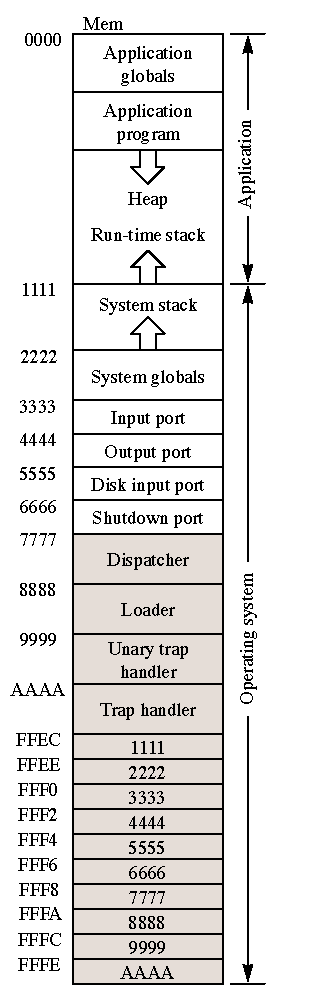
\includegraphics{pep10-memory-map}
\end{center}

\newpage

\fancyhf[ORH,ERH]{\bfseries \sffamily CPU data section}
\noindent Here is the data section of the Pep/10 CPU.
Compared to the Pep/9 data section, Pep/10 has two additional components -- a shadow carry bit, denoted S in the figure below, and an additional multiplexer with its associated control line CSMux.
The shadow carry bit is not visible at the ISA level and is used for internal address calculations in the microcode.
This design solves a major headache present in Pep/9, which requires the saving and restoration of the C bit when an internal address addition would wipe it out.
A step towards a more realistic model is the requirement of three consecutive MemRead/MemWrite assertions for memory access as opposed to two with Pep/9.\\
\begin{center}
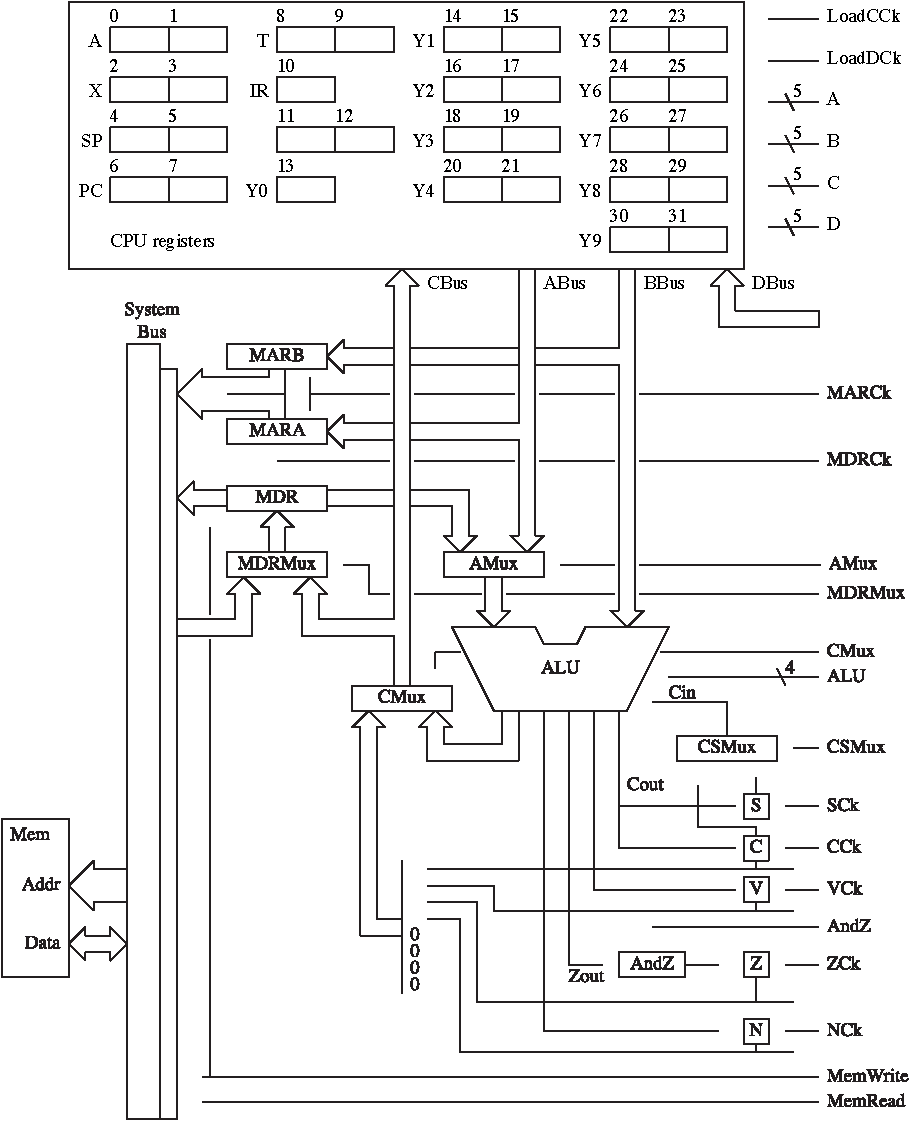
\includegraphics{pep10-1-byte-bus}
\end{center}

\newpage

\fancyhf[ORH,ERH]{\bfseries \sffamily CPU data section with two-byte data bus}
\noindent Here is the data section of the Pep/10 CPU with the two-byte data bus.
The fifth edition of \textit{Computer Systems} drops the discussion of the MAR Incrementer in favor of a more extensive discussion of increasing the data bus width to improve performance.
The material is improved by incorporating it into the Pep9CPU software.
Students can toggle between the two models, with and without the wider data bus, test their solutions with the software, and use the UnitPre and UnitPost tests in the Help system.

\begin{center}
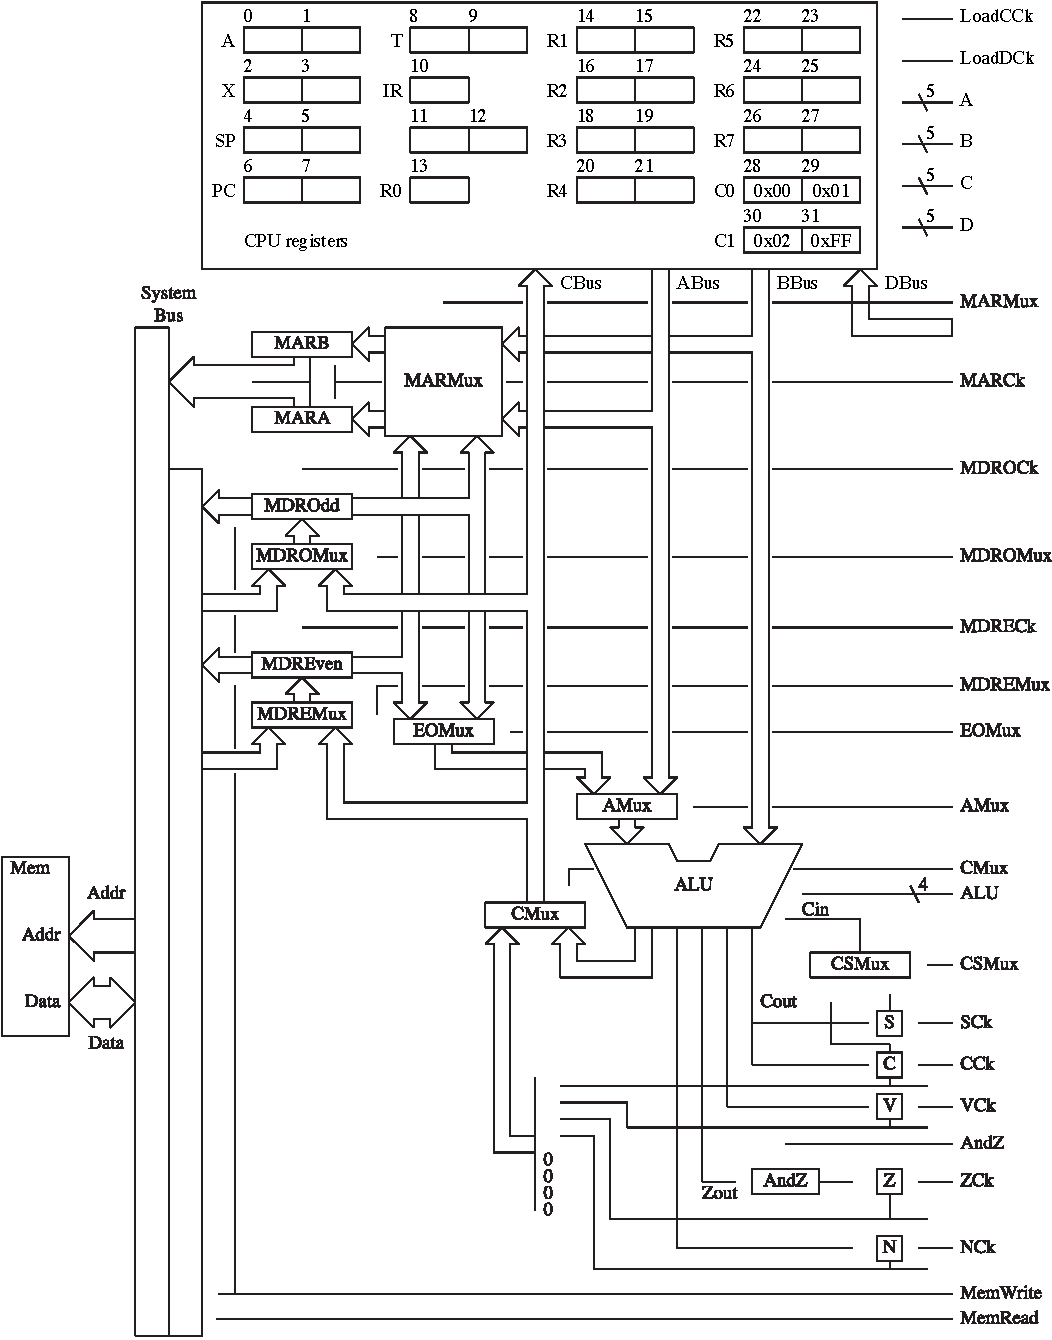
\includegraphics[scale=0.95]{pep10-2-byte-bus.pdf}
\end{center}

\end{document}
